\documentclass{article}
\usepackage{amsmath}
\usepackage{graphicx}  % For including images
\usepackage{hyperref}  % For hyperlinks

\begin{document}

\title{CS276 Homework 1: Light Field Rendering}
\author{Zhaoyu Qiu 2024192955\\ School of Biomedical Engineering \\ ShanghaiTech University }
\date{\today}
\maketitle

\section{Introduction}
The purpose of this assignment is to perform refocusing based on light field data and to experiment with different aperture effects. The input for this assignment is a 16x16 image matrix, referencing classic projects such as Lytro camera data processing.

\section{Implement}

\subsection{Light Field Loading}
The 16x16 light field input used for the text is shown in Figure \ref{fig:light_field}.

\begin{figure}[ht]
    \centering
    \includegraphics[width=.7\textwidth]{./light_field_matrix.png}  % Replace with your image path
    \caption{16x16 Light Field Input}
    \label{fig:light_field}
\end{figure}

To create a light field, multiple images are captured from various viewpoints and organized into a 5D data structure, represented as:
\[
\text{Light Field}(u, v, x, y, c)
\]
where \( (u, v) \) represent the camera indices, \( (x, y) \) are the pixel coordinates, and \( c \) denotes the color channels. Each image is resized and stored in the array, ensuring uniform dimensions for accurate interpolation.

\subsection{Interpolation Resampling}
Interpolation is a crucial step in rendering the light field. Two primary interpolation methods are employed:

\subsubsection{Bilinear Interpolation}
For bilinear interpolation, the pixel value \( I(x, y) \) at an arbitrary position is calculated using:
\[
I(x, y) = w_a \cdot I_a + w_b \cdot I_b + w_c \cdot I_c + w_d \cdot I_d
\]
where \( w_a, w_b, w_c, w_d \) are the weights based on the neighboring pixel values.

\subsubsection{Trilinear Interpolation}
In a 3D light field, trilinear interpolation is utilized, which extends the bilinear approach into the depth dimension. The formula is given by:
\begin{align*}
    I(x, y, z) = & \, I_{000}(1-x)(1-y)(1-z) + I_{100}(x)(1-y)(1-z)\\
                  & \, + I_{010}(1-x)(y)(1-z) + I_{110}(x)(y)(1-z) \\
                  & \, + I_{001}(1-x)(1-y)(z) + I_{101}(x)(1-y)(z) \\
                  & \, + I_{011}(1-x)(y)(z) + I_{111}(x)(y)(z)
    \end{align*}
    

\subsection{Focal Plane Control}
Let the camera position be \( C = (x_c, y_c) \) and the focus distance be \( f \). The distance from a pixel point \( P = (x, y) \) to the camera position is calculated as:
\[
d = \sqrt{(x - x_c)^2 + (y - y_c)^2}
\]
The weight \( w \) for each camera view can be computed using the Gaussian function:
\[
w = \frac{1}{\sigma \sqrt{2\pi}} e^{-\frac{d^2}{2\sigma^2}}
\]
where \( \sigma \) is related to the aperture size, influencing the weight distribution.

\subsection{Aperture Control}
Let \( A \) be the aperture size, which affects the weight calculation. A larger aperture allows more camera views to contribute to the final image. The relationship can be described as:
\[
w \propto \frac{1}{A}
\]
This means that as the aperture increases, the weight distribution becomes flatter, impacting the clarity and detail of the final image.

\subsection{Z-Axis Control}
The focal length factor \( F \) simulates depth along the z-axis. The displacement in the x and y directions for each camera view can be calculated as:
\[
dx = (col - x_c) \cdot F \cdot \frac{width}{f}
\]
\[
dy = -(row - y_c) \cdot F \cdot \frac{height}{f}
\]
Here, \( (col, row) \) represents the position of the camera view, and \( (width, height) \) are the dimensions of the final image. The blur effect in the final image is controlled by the kernel size:
\[
\text{blur\_kernel\_size} = \max(1, \text{int}(F \cdot 2))
\]

\section{Experiments}
\subsection{GUI interface}
The user interface of this assignment consists of the components shown in the Figure \ref{fig:ui}, which includes 6 control sliders, 1 display page, and 1 confirm button.

\begin{figure}[h]
    \centering
    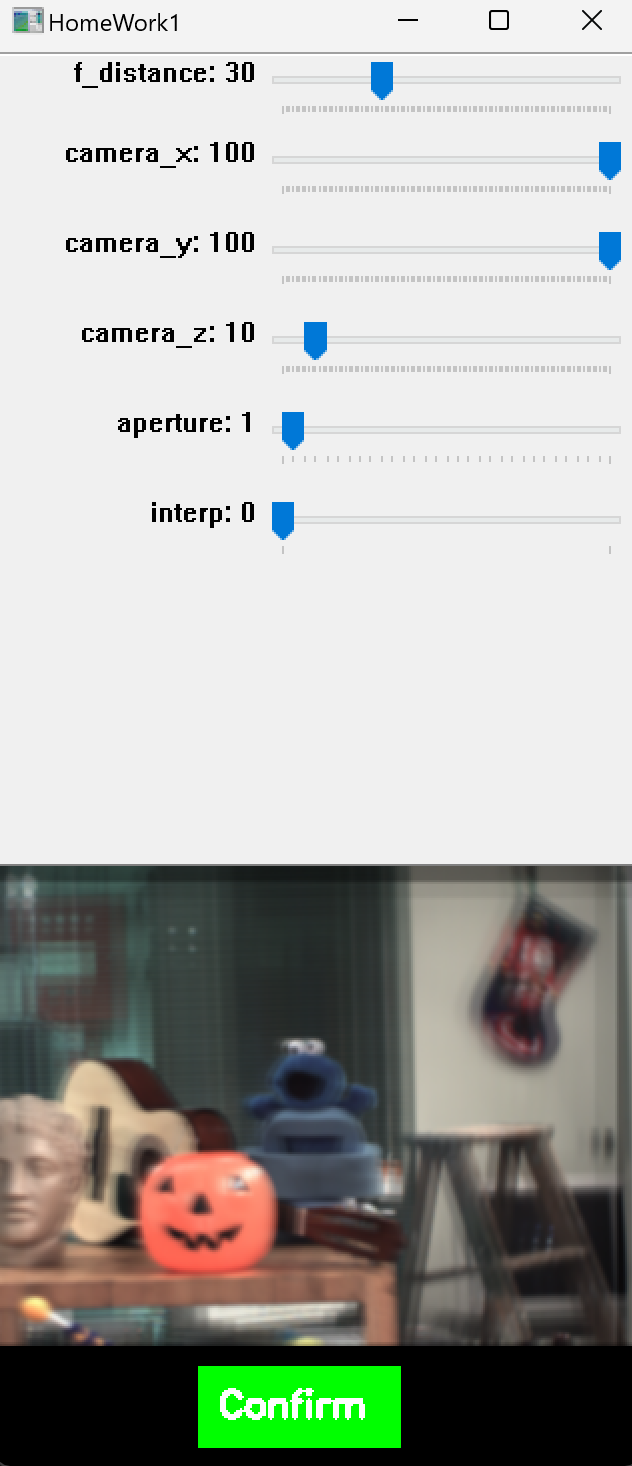
\includegraphics[width=0.25\textwidth]{GUI.png} % 替换为你的图片路径
    \caption{User Interface Overview}
    \label{fig:ui}
\end{figure}

\subsection{Interpolation Resampling}


\subsection{Focal Plane Control}

\subsection{Aperture Control}

\subsection{Z-Axis Control}


\section{Conclusion}
This work presented a comprehensive overview of light field rendering, detailing the underlying principles and implementation techniques. The experiments highlighted the benefits of using advanced interpolation methods and the impact of camera parameters on rendering quality. Future work will explore more complex scenes and real-time rendering capabilities, further enhancing the interactive experience in light field visualization.

% If you have references, you can include them here:
\begin{thebibliography}{9}
    \bibitem{reference1} 
    Author, A. (Year). 
    \textit{Title of the paper}. Journal Name, Volume(Issue), Page range.
    
    % Add more references as needed
\end{thebibliography}

\end{document}
